\usepackage{xcolor}
\usepackage{afterpage}
\usepackage{pifont,mdframed}
\usepackage[bottom]{footmisc}
\usepackage{minted}

\createsection{\Grader}{Grader di prova}
\newcommand{\inputfile}{\texttt{stdin}}
\newcommand{\outputfile}{\texttt{stdout}}
\makeatletter
\renewcommand{\this@inputfilename}{\texttt{stdin}}
\renewcommand{\this@outputfilename}{\texttt{stdout}}
\renewcommand{\this@syllabuslevel}{5}
\renewcommand{\this@custdifficulty}{3}
\makeatother

% % % % % % % % % % % % % % % % % % % % % % % % % % % % % % % % % % % % % % % % % % %
% % % % % % % % % % % % % % % % % % % % % % % % % % % % % % % % % % % % % % % % % % %
Finito l'anno scolastico, Marco è più che felice di godersi le sue meritate vacanze estive!
Dopo poco però, si rende conto di aver ben poco da fare, e decide di scaricare un nuovo gioco sul cellulare.
Il gioco si chiama \textit{Squaremania} e consiste nel formare un quadrato a partire da
$N$ blocchi di legno di dimensione $1\times1$.
Ovviamente, non è possibile rompere o tagliare i blocchi in alcuna maniera.

\begin{figure}[h]
    \centering
    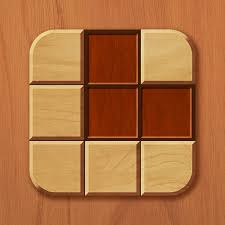
\includegraphics[width=0.4\textwidth]{./woodoku.jpg}
    \caption{L'icona di \textit{Squaremania}, totalmente non copiata da un altro gioco.}
\end{figure}

È possibile ottenere un quadrato? Se sì, Marco vuole sapere la dimensione del lato, altrimenti scrivi \texttt{NO}.


\Implementation

Dovrai sottoporre un unico file, con estensione \texttt{.cpp}.

\begin{warning}
    Tra gli allegati a questo task troverai un template \texttt{squaremania.cpp} con un esempio di implementazione.
\end{warning}

Il file di input è composto da $1$ riga:
\begin{itemize}
    \item Riga 1: l'intero $N$.
\end{itemize}

Il file di output è composto da $1$ riga:
\begin{itemize}
    \item Riga 1: La lunghezza del lato del quadrato (solo se è possibile formarlo), altrimenti \texttt{NO}.
\end{itemize}

% % % % % % % % % % % % % % % % % % % % % % % % % % % % % % % % % % % % % % % % % % %
% % % % % % % % % % % % % % % % % % % % % % % % % % % % % % % % % % % % % % % % % % %

\Constraints

\begin{itemize}[nolistsep, itemsep=2mm]
    \item $1 \le N \le 1\:000\:000$.
\end{itemize}

% % % % % % % % % % % % % % % % % % % % % % % % % % % % % % % % % % % % % % % % % % %
% % % % % % % % % % % % % % % % % % % % % % % % % % % % % % % % % % % % % % % % % % %

\Scoring

Il tuo programma verrà testato su diversi test case raggruppati in subtask.
Per ottenere il punteggio relativo ad un subtask,
è necessario risolvere correttamente tutti i test che lo compongono.

\IIOTsubtask{0}{1}{Casi d'esempio.}

\IIOTsubtask{50}{1}{$N \le 1\:000$}

\IIOTsubtask{50}{1}{Nessuna limitazione aggiuntiva.}


% % % % % % % % % % % % % % % % % % % % % % % % % % % % % % % % % % % % % % % % % % %
% % % % % % % % % % % % % % % % % % % % % % % % % % % % % % % % % % % % % % % % % % %

\Examples

\begin{example}
    \exmpfile{squaremania.input0.txt}{squaremania.output0.txt}%
    \exmpfile{squaremania.input1.txt}{squaremania.output1.txt}%
    \exmpfile{squaremania.input2.txt}{squaremania.output2.txt}%
\end{example}

% % % % % % % % % % % % % % % % % % % % % % % % % % % % % % % % % % % % % % % % % % %
% % % % % % % % % % % % % % % % % % % % % % % % % % % % % % % % % % % % % % % % % % %

\Explanation

Nel primo esempio, con un cubetto si può formare un quadrato $1\times1$.

Nel secondo esempio, con $9$ cubetti si può formare un quadrato $3\times3$.

Nel terzo esempio non è possibile formare un quadrato.